\subsection{10.8 Formen von Quadriken}{
\vskip1pt

Je nach Rang von A, den Vorzeichen der EW von $A$, $a$ und $b$ ergeben sich verschiedenen Typen von von Kegelschnitten respektive Quadriken.\par\vskip4pt

\textbf{Ellipse}\par\vskip2pt
$q(x) = a^2x_1^2 + b^2x_2^2 = 1$

\vspace{-2.5mm}
\begin{center}
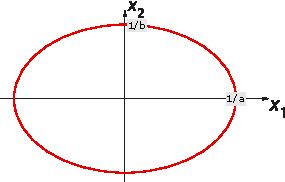
\includegraphics[width=0.45\columnwidth]{10_Quadratische_Formen/ellipse.pdf}
\end{center}
\vspace{-2mm}

\textbf{Hyperbel}\par\vskip2pt
$q(x) = a^2x_1^2 - b^2x_2^2 = 1$

\vspace{-2mm}
\begin{center}
\begin{minipage}{0.4\columnwidth}
	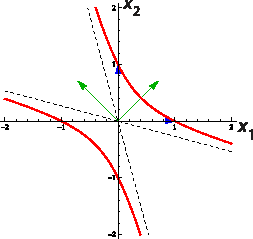
\includegraphics[width=\textwidth]{10_Quadratische_Formen/hyperbel.pdf}
\end{minipage}
\hspace{1em}%\hfill
\begin{minipage}{0.3\columnwidth}
	\textcolor{blue}{Standardbasis}\par
	\textcolor{OliveGreen}{Hauptachsenbasis}\par
	\textcolor{red}{Hyperbel}\par
	Asymptoten: $\pm\frac{a}{b}$
\end{minipage}
\end{center}
\vspace{-2mm}

\textbf{Weitere Formen}\par\vskip2pt
\begin{tabular}{ll}
	$a^2x_1^2 + b^2x_2^2 + 1 = 0$ & leere Menge \\
	$x_1^2 + b^2x_2^2 = 0$        & Punkt \\
	$x_1^2 - b^2x_2^2 = 0$        & sich schneidendes Geradenpaar \\
\end{tabular}

}
\WhiteSpace